\documentclass[a4paper,10pt,twoside]{IEEEtran}

\usepackage{graphicx}
\usepackage{placeins}
\usepackage{hyperref}
\usepackage{pdfpages}
\usepackage{fullpage}
\usepackage[bf]{caption}
\usepackage[english]{babel}
\usepackage{verbatim}
\usepackage{cite}
\usepackage{wrapfig}
\usepackage[marginpar]{todo}
\usepackage{paralist}
\usepackage{booktabs}
\usepackage{subcaption}
\usepackage{mathtools}
\usepackage{fancyhdr}
\usepackage{algpseudocode}
\usepackage{algorithm}
\usepackage{tikz}
%\usepackage{gnuplot-lua-tikz}
\usetikzlibrary{calc,intersections}
\usepackage{amssymb}

\hypersetup{
    colorlinks,
    pdftitle={Report Localization Option 1 IN4254 Smart Phone Sensing},
    pdfauthor={in4254-dhoepelman-mprovokluit},
}

\setlength{\parindent}{0pt}
\setlength{\parskip}{2ex}

\usepackage[utf8]{inputenc}
\usepackage[T1]{fontenc}

\newcommand{\axis}[1]{$#1$\nobreakdash-axis}
\newcommand{\plane}[2]{$#1#2$\nobreakdash-plane}

\title{\huge{\textbf{Report Localization Option 1}\\IN4254 Smart Phone Sensing}}
\date{\today}
\author{David Hoepelman (1521969) \and Mark Provo Kluit (1263099)}

\setlength{\headheight}{15pt}
\addtolength{\headsep}{15pt} % no love between header and main text
%\addtolength{\textheight}{-20pt} % more space between text and empty footer

\pagestyle{fancy}
 
\fancyhf{}
\fancyhead[LE,RO]{\thepage}
\fancyhead[RE]{\textit{\nouppercase{\leftmark}}}
\fancyhead[LO]{\textit{\nouppercase{\rightmark}}}
 
\fancypagestyle{plain}{ %
\fancyhf{} % remove everything
\renewcommand{\headrulewidth}{0pt} % remove lines as well
\renewcommand{\footrulewidth}{0pt}}

\begin{document}

\maketitle

\section{Data collection}
\label{sec:localization-method}

For each of the available 17 rooms on the 9$^{\text{th}}$ floor of EWI, we have collected Wi-Fi signal strengths of all the access points our mobile phone could find.
We have drawn a rough not-to-scale map of the rooms, and show it to the user as part of our GUI. See \autoref{fig:screenshot}.

\begin{figure}
  \centering
    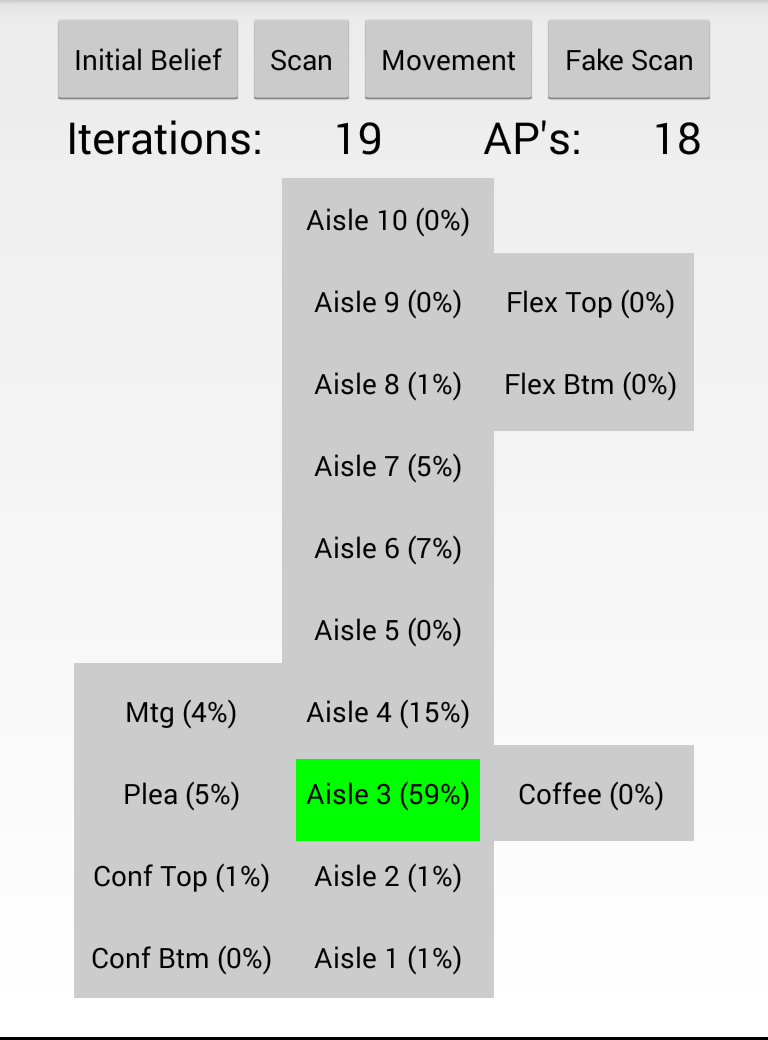
\includegraphics[width=0.36\textwidth]{screenshot}
    \caption{GUI showing successful localization}
    \label{fig:screenshot}
\end{figure}

In total we have collected \textbf{3300} scans on three different days.
A scan list contains the \emph{access points} (AP's) that were detected as a list of $signal = (BSSID, SSID, level)$ tuples where $level$ is expressed in dBm with a range of $[-30,-100]$.
Both 2.4~Ghz and 5~Ghz access points were detected and stored in the database.
Most rooms have either 180 or 240 scans, depending on which days they were accessible.
The collected scans inside a room were evenly divided among the room area.

On average each scan contains 20~$BSSID$'s, although the number varies per room.
We did a fixed number of scans per room on every day, but this does not translate well into a sampling time per cell.
The reason for this is that the time required to perform a signal scan
differs greatly depending on the number of AP's that are visible in a room.

\section{Localization method}
\label{sec:data}

We chose to use \textbf{Bayesian Filters} for our localization method. We uniquely identify an AP using the $BSSID$, which is guaranteed globally unique.

For our calculations we group the training data on $BSSID$ and $Room$ and calculate the normal distribution $N_{BSSID,Room}(\mu_{BSSID,Room}, \sigma^2_{BSSID,Room})$ using the measured signal strengths.

Signals whose $SSID$ is either ``TUvisitor'', ``tudelft-dastud'',
or ``Conferentie-TUD'' are ignored.
This is because most access points of the TU Delft sent out four different $SSID$'s (the fourth is ``eduroam'') with different $BSSID$'s.
As these signals come from the same physical location and have the same
frequency (and probably the same radio's) we did not think they would add more
information, and at worst might make our results less accurate (by processing
essentially the same signal 4 times, thus biasing the results heavily on those AP's).

For localization we express the location as a probability vector $\mathbf{loc}$, with $\mathbf{loc}_{r}$ being the probability that we are in room $r$. 
We initially start with the \emph{intial belief} where all locations have the same probability $\mathbf{loc}_r = \frac{1}{|\mathbf{loc}|}$.
We then do a WiFi scan which gives a list of signals.
We sort this list on level, with strongest level first.
As long as the largest probability is under a threshold $0.95$ we then iterate the list, while adjusting the location each iteration.
The location is adjusted by getting for each room the chance of that signal level and multiplying it with the existing probability. After each iteration we normalize $\mathbf{loc}$ by making it sum to 1.
\\
\begin{algorithmic}
	\State $scan \gets \text{list of } (BSSID, SSID, level) \text{ sorted on }level$
	\While {$\max\left(\mathbf{loc}\right) < 0.95$}
		\State $signal \gets \text{next}\left(scan\right)$
		\ForAll{$Room$}
			\State $p \gets N_{BSSID,Room}(level-0.5,level+0.5)$
			\State $\mathbf{loc}_{Room} \gets \mathbf{loc}_{Room} \cdot p $
		\EndFor
		\State $\text{normalize}\left(\mathbf{loc}\right)$
	\EndWhile
\end{algorithmic}

$\mathbf{loc}$ is retained between scans until the locator is reset by the user to its initial belief.

\subsection{Number of access points}
\label{subsec:numap}

While we achieved a pretty good accuracy with pure bayesian filters (see performance evaluation section), we had trouble in the \emph{Coffee} room which did not have a large number of APs visibile, thus providing too little information for our bayesian filter.
We solved this problem by constructing $N_{\#,Room}$ distributions.
This distribution gives the probability for number of AP's in a scan based on the $\mu$ and $\sigma$ of the number of AP's per room in the training data.
Thus we append the following to the previous algorithm:
\\
\begin{algorithmic}
	\If {$\max\left(\mathbf{loc}\right) < 0.95$}
		\ForAll{$Room$}
			\State $p \gets N_{\#,Room}(|scan|-0.5,|scan|+0.5)$
			\State $\mathbf{loc}_{Room} \gets \mathbf{loc}_{Room} \cdot p $
		\EndFor
		\State $\text{normalize}\left(\mathbf{loc}\right)$
	\EndIf
\end{algorithmic}

\section{Performance evaluation}
\label{sec:evaluation}

For our performance evaluation we used off-line processing. We divided the scans of our training data into 10 random partitions, and tested every partition while using the other partitions as training data for the locator.

Using this method we achieved an accuracy of \textbf{83\%} (2731 correct out of 3300).
While analyzing the data we saw that a lot of the mis-classified scans occurred in the Coffee room,
where a scan usually contains at most three signals. This is not enough for the bayesian filter.

To alleviate this problem we altered our code to take the number of visible signals into account.
This improved our accuracy to \textbf{89\%} (2945 of 3300).
The technical implementation for this is specified in section \ref{subsec:numap}.
If we mark adjacent rooms as correct too, which is not unreasonable as some training scans were taken on the border between rooms, the accuracy increases to \textbf{95\%} (3132 of 3300).

\section{Discussion}
\label{sec:discussion}
TODO

Bayesian filters are not that useful if you have rooms with only a low number of visible access points.
Our trick to take the number of AP's into accounts works well when there
are not too many rooms with few visible AP's.
However, if there are more rooms like the Coffee room, this approach will likely fail.
Another possibility we contemplated was to create a bitstring of present/not-present $BSSID$'s for the current scan and the training data.
Computing the hamming distances to the training data points increases the amount of information that
is available to the filter, thus possibly increasing the accuracy.
This will more likely work in the general case.

%\newpage

%\addcontentsline{toc}{chapter}{Bibliography}
% styles: abbrv, ieeetr, plain
%\bibliographystyle{abbrv}
%\bibliography{report}

\newpage
\appendix

\end{document}
